\documentclass[12pt, a4paper]{article}
\usepackage[utf8]{inputenc}
\usepackage{enumitem}
\usepackage{amsmath, amssymb, amsthm}
\usepackage{graphicx}
\usepackage[export]{adjustbox}
\usepackage{xcolor}
\graphicspath{ {./img/} }

\title{%
51.504 Machine Learning (2020) \\
Lecture Note 03: Classification}
\date{2020-10-01}
\author{%
Jon Kartago Lamida}

\begin{document}
  \maketitle
  \setlength{\parindent}{0pt}

\section*{Examples}
\begin{itemize}
  \item Tumor Classification
  \item Spam Filters
\end{itemize}


\section*{Methodology}
Machine Learning \texttt{>} Supervised Learning \texttt{>} Classification
\begin{itemize}
  \item \textbf{Task}. \( h: \mathbb{R}^d \rightarrow \{-1, +1\} \) such that \( y \approx h(x; \theta)  \)
  \item \textbf{Experience}. Training data \( (x^{(1)}, y^{(1)}), \dots, (x^{(n)}, y^{(n)})  \)
  \item \textbf{Performance}. Prediction error on test data
\end{itemize}

\section*{Gradient Descent}
The slope at a  point is called the \emph{derivative} at that point \\

Intuition: Measure the slope between two points that are really close together \\

\( \dfrac{f(x + c) - f(x)}{c} \)

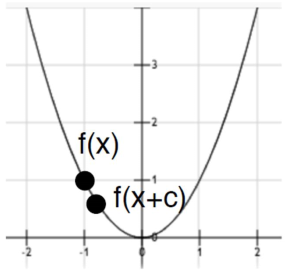
\includegraphics[scale=0.5]{gradient-descend}

Limit as \( c \) goes to zero

\section*{Linear Classifier}
\subsection*{Methodology}

\section*{Model}

\section*{Test Loss}

\section*{Decision Region}

\section*{Linearly Separable}

\section*{Not Linearly Separable}

\section*{Perceptron Algorithm}
Linear classifiers are often also called perceptrons.

\section*{Zero-One Loss}

\section*{Training Loss}

\section*{Hypothesis Function}
The hypothesis function is given by \\
\\
\( h_\theta\bigg(x^{(i)}\bigg) = sgn\bigg(\bigg\langle\theta,x{(i)}\bigg\rangle\bigg) \), \\
where \\
\\
\( 
  sgn(z) = {
    \begin{cases}
    1 & if z \geq 0 \\
    -1 & if z <
  \end{cases}
}  
\)

\section*{Loss Function}

\section*{Perceptron Algorithm}

\section*{Error Reduction}

\section*{Perceptron Summary}

\section*{Convergence}
\subsection*{Example}

\section*{Disadvantages}

\section*{Logistic Regression}

\section*{Almost Linearly Separable}

\section*{Sigmoid Neuron}

\section*{Probabilistic Model}

\section*{Sigmoid Function}

\section*{Solving for Hyperlapse}

\section*{Decision Boundary}

\section*{Sigmoid Function Formulas}

\section*{LOG-Likelihood Function}

\section*{Gradient}

\section*{Gradient Ascent}

\section*{Multiclass Classification}

\end{document}